\documentclass{standalone}
\usepackage{pgfplots}
\usepackage{tikz}
\usepackage{amsmath}
\usepackage{relsize}
\pgfplotsset{compat = 1.3}

\begin{document}
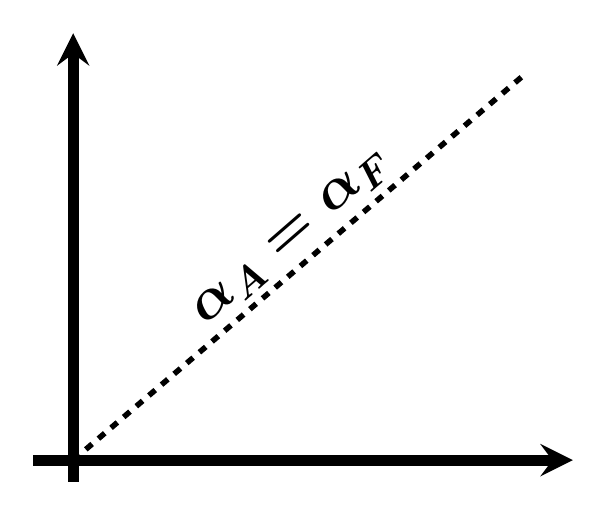
\begin{tikzpicture}
  \begin{axis}[ 
    xlabel={},
    ylabel={},
    xmin=-0.08,
    xmax=1,
    ymin=-0.05,
    ymax= 1,
    axis x line*=bottom,
    axis y line*=left,
    ticks=none,
    enlargelimits = true,
    axis lines=middle,
    axis line style={line width=4pt},
  ] 
    \addplot[dashed, line width=2pt][domain=0:0.9] {x};
    \addplot[mark=none] table[row sep=crcr] {0.44 0.52\\} node[rotate=41] {\huge $\boldsymbol{\alpha_{A} = \alpha_{F}}$};
    
  \end{axis}
\end{tikzpicture}


\end{document}